% Source data and model: vicioms/eq_thinfilm,
% commit 2669ac297713cf9ad6908b45ac056d583dd2affa.
\section{Model and observables}
\label{sec:model}

We consider a two-dimensional scalar order parameter $\phi(\boldsymbol r,t)$ with
overdamped dynamics
\begin{equation}
 \partial_t\phi=\nabla^2\phi+\phi-\phi^3+F+\eta_a(\boldsymbol r).
 \label{eq:model}
\end{equation}
The Laplacian is the nearest-neighbour lattice Laplacian.
The force $F$ favours the phase $\phi>0$.
The quenched random force $\eta_a$ is Gaussian with zero mean.
For a lattice of $N$ sites, define
$\eta_{a,\boldsymbol k}=\sum_{\boldsymbol r}
\eta_a(\boldsymbol r)e^{-i\boldsymbol k\cdot\boldsymbol r}$.
Its covariance is
\begin{equation}
 \mathbb E[\eta_{a,\boldsymbol k}\eta_{a,\boldsymbol k'}^*]
 =N\Delta^2\frac{f_a(\boldsymbol k)}{\mathcal N_a}
 \delta_{\boldsymbol k,\boldsymbol k'},
 \qquad
 \mathcal N_a=\frac{1}{N}\sum_{\boldsymbol k}f_a(\boldsymbol k),
 \label{eq:noise-covariance}
\end{equation}
where $\mathbb E$ denotes the disorder average. We compare isotropic
and anisotropic disorder with
\begin{align}
 f_0(\boldsymbol k)&=k\,e^{-k^2w^2},
 & &\text{isotropic},\nonumber\\
 f_1(\boldsymbol k)&=
 \frac{2(\boldsymbol k\cdot\hat{\boldsymbol b})^2}{k}
 e^{-k^2w^2},
 & &\text{anisotropic},
 \label{eq:two-disorders}
\end{align}
for $k=|\boldsymbol k|>0$, and $f_a(\boldsymbol 0)=0$.
The unit vector $\hat{\boldsymbol b}=(\cos\beta,\sin\beta)$ fixes the
anisotropy axis. Intermediate anisotropies are defined by
$f_a=(1-a)f_0+af_1$, with $0\leq a\leq1$.
The normalization gives $\mathbb E[\eta_a(\boldsymbol r)^2]=\Delta^2$.
We use $\Delta=0.04$, $w=3$ and unit lattice spacing.

We retain the dominant interface contour
$\boldsymbol r(s)=(x(s),y(s))$, including overhangs, with arc length
$s\in[0,P)$. Its length is $P=\int_\Gamma d\ell$.
For flat interfaces we use one spatial period and set $h_s(s)=y(s)$.
For bubbles we use the closed outer contour and set
$h_s(s)=|\boldsymbol r(s)-\boldsymbol c|$, where $\boldsymbol c$ is the
area centroid enclosed by that contour.
In both geometries, $s$ is sampled uniformly and the mean height is
subtracted. For a scalar profile $h(u)$ of period $T$, define
\begin{equation}
 \langle h\rangle_T=\frac{1}{T}\int_0^T h(u)\,du,
 \qquad
 \widehat h_n=\frac{1}{T}\int_0^T
 [h(u)-\langle h\rangle_T]e^{-2\pi inu/T}\,du,
 \qquad
 q_n=\frac{2\pi n}{T}.
 \label{eq:height-modes}
\end{equation}
The single-contour spectrum is $S_i(q_n)=T|\widehat h_n|^2$,
with $T=P_i$ for the arc-length profile.
We average spectra over disorder realizations in common physical $q$
bins, first averaging modes within each contour and then giving equal
weight to each contour. Bins are merged until every contour contributes.
This treats the fluctuating contour length $P_i$ explicitly.
The quoted exponents are fitted to these binned spectra.
The figures show instead $S(n)=\langle|\widehat h_n|^2\rangle$ at fixed
mode index $n\geq2$, again with equal weight per contour.

\section{Flat interfaces}
\label{sec:flat}

The system is periodic along $x$, has height $L_y=2L_x$, and contains
a single interface with $\phi>0$ below it. The force $F$ is increased
quasistatically, and the last pinned configuration before the interface
reaches the upper boundary is retained. We call this the depinning configuration.
One period satisfies
$\boldsymbol r(P)=\boldsymbol r(0)+(L_x,0)$.

We also construct an area-preserving profile.
If a column intersects the dominant contour at ordered heights
$y_1<\cdots<y_{2m+1}$, its height is
\begin{equation}
 h_x(x)=\sum_{j=1}^{2m+1}(-1)^{j+1}y_j(x),
 \qquad x\in[0,L_x).
 \label{eq:area-height}
\end{equation}
This is the occupied height below the contour in that column.
Detached islands and hole boundaries are omitted.

\subsection{Isotropic disorder}
\label{sec:flat-isotropic}

For $a=0$ we analyse $256,128,64,32$ realizations at
$L_x=256,512,1024,2048$, respectively.
Figure~\ref{fig:flat-profiles} shows the contour, $h_x(x)$ and $h_s(s)$
for the same realization.

\begin{figure}[H]
 \centering
 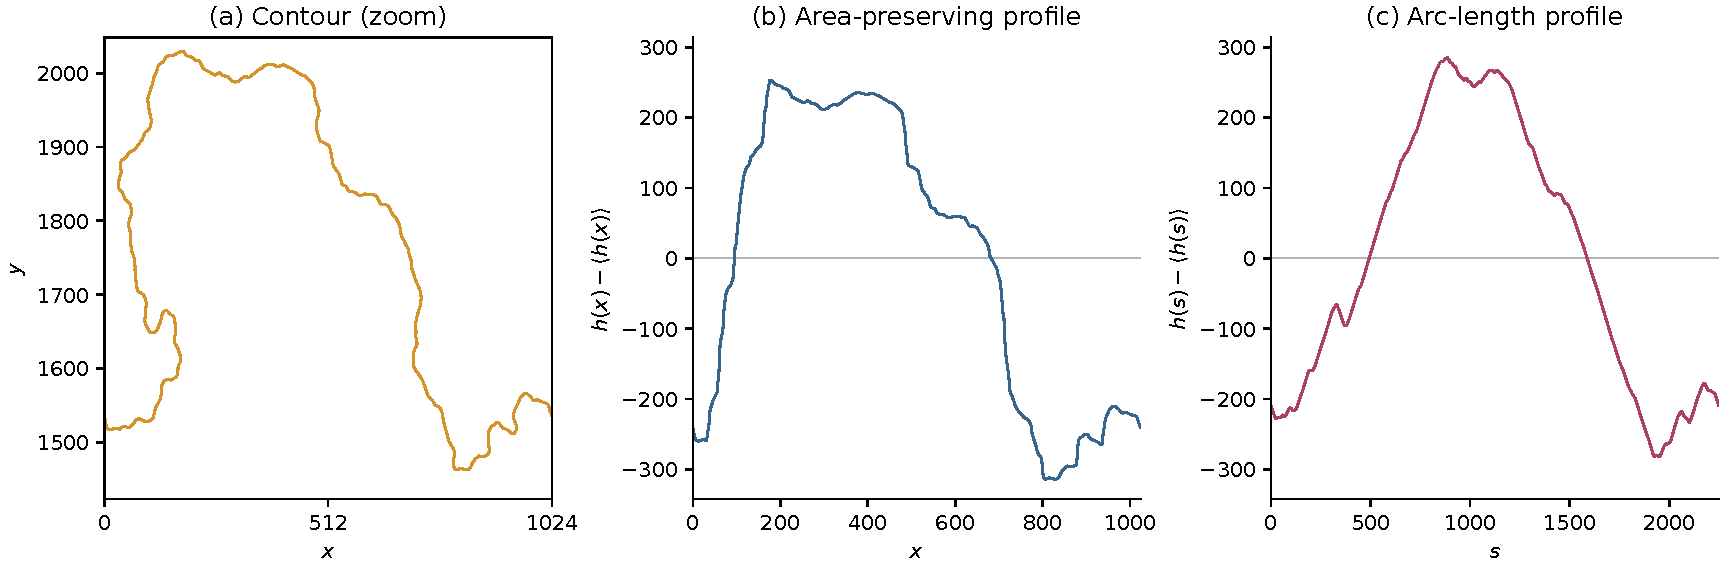
\includegraphics[width=\linewidth]{fig1_profiles.pdf}
 \caption{Flat interface with isotropic disorder at $L_x=1024$,
 with contour length $P=2248.42$.
 (a) Enlarged view of the full depinning contour.
 (b) Area-preserving profile $h(x)$, defined from the alternating sum
 of the crossing heights in each column.
 (c) Height $h(s)=y(s)$ along the contour, parametrized by arc length
 $s\in[0,P)$.
 In (b,c), the means $\langle h(x)\rangle$ and
 $\langle h(s)\rangle$ are subtracted, respectively.}
 \label{fig:flat-profiles}
\end{figure}

The mean perimeter grows approximately as
$\mathbb E[P]\propto L_x^{1.22}$.
Figure~\ref{fig:flat-scaling}(a) compares this growth with $L_x$
and $L_x^{1.25}$.
For a self-affine interface, the qEW exponent
$\zeta=1.25$ corresponds to $S(n)\propto n^{-3.5}$.
Figure~\ref{fig:flat-scaling}(b) shows $S(n)$ for the two largest sizes.
Over all the modes shown, the arc-length spectra decay as
$n^{-(1+2\zeta)}$ with $\zeta\simeq1.15$ at $L_x=1024$ and $1.06$ at
$L_x=2048$, more slowly than the qEW line.
The $h_x$ spectra are flatter, with $\zeta\simeq0.95$ and $0.81$.

\begin{figure}[H]
 \centering
 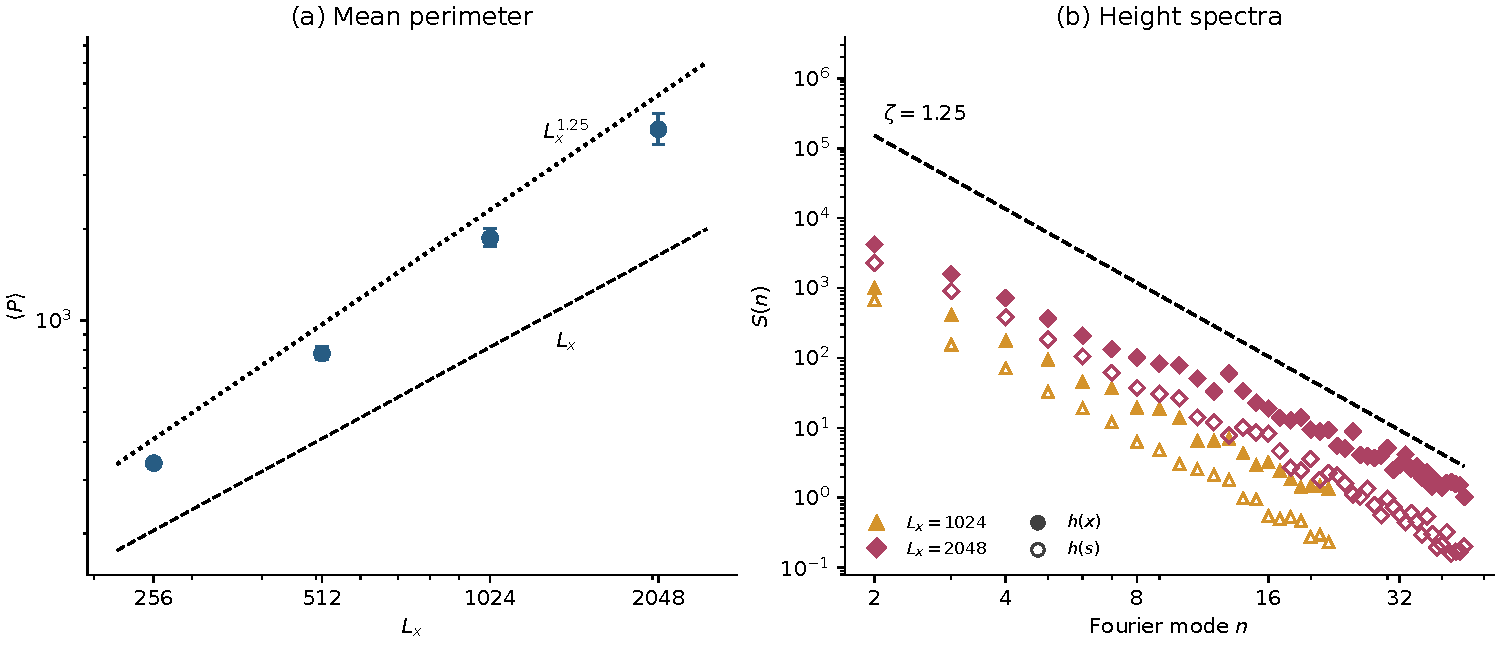
\includegraphics[width=\linewidth]{fig2_scaling.pdf}
 \caption{Isotropic flat interfaces with $L_y=2L_x$.
 (a) Mean perimeter versus $L_x$.
 Error bars give $95\%$ bootstrap intervals for the mean.
 The black dashed and dotted lines have slopes $1$ and $1.25$, respectively.
 (b) Spectra $S(n)=\langle|\widehat h_n|^2\rangle$ versus the mode
 index $n$ for $L_x=1024$ and $2048$, with $2\leq n\leq45L_x/2048$.
 Filled symbols represent $h_x(x)$ and open symbols represent $h_s(s)$.
 The black dashed line has slope $-3.5$ ($\zeta=1.25$), with a freely
 chosen amplitude.
 Each contour has equal weight in the disorder average.}
 \label{fig:flat-scaling}
\end{figure}
